\documentclass[10pt,a4paper]{report}
\usepackage[utf8]{inputenc}
\usepackage[russian]{babel}
\usepackage{amsmath}
\usepackage{amsfonts}
\usepackage{amssymb}
\usepackage{graphicx}
\author{Скрипаль Борис}
\title{Лабораторная работа №1.\\
	Программа для шифрования и подписи GPG, пакет Gpg4win}
\begin{document}
\maketitle
\tableofcontents
\pagebreak

\section{Цель работы}
Научиться создавать сертификаты, шифровать файлы и ставить ЭЦП.
\section{Описание лабораторной работы}
Электронная цифровая подпись (ЭЦП) — реквизит электронного документа, полученный в результате криптографического преобразования информации с использованием закрытого ключа подписи и позволяющий проверить отсутствие искажения информации в электронном документе с момента формирования подписи (целостность), принадлежность подписи владельцу сертификата ключа подписи (авторство), а в случае успешной проверки подтвердить факт подписания электронного документа (неотказуемость).

В данной лабораторной работе для генерации ЭЦП будет использоваться набор утилит, реализующих стандарт OpenPGP (Kleopatra, GPG4win и др.).
\section{Ход работы}
\subsection{Создание сертификата openPGP}
Для создания новой ключевой пары OpenPGP необходимо открыть графическую оболочку \textit{"Kleopatra"} и выполнить команду \textit{"File \begin{math}\to\end{math} New Certificate"}. После чего откроется помощник (рисунок \ref{ris:step11}).

\begin{figure}[h]
	\center{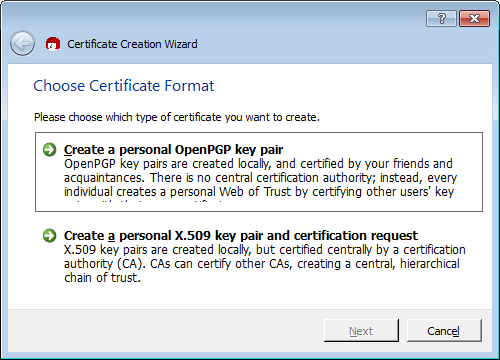
\includegraphics[width=1\linewidth]{res/step11}}
	\caption{Окно выбора типа сертификата безопасности.}
	\label{ris:step11}
\end{figure}

В данном случае необходимо выбрать первый пункт (\textit{Create a personal OpenPGP key pair}), после чего откроется окно ввода информации о пользователе (рисунок \ref{ris:step12}).

\begin{figure}[h]
	\center{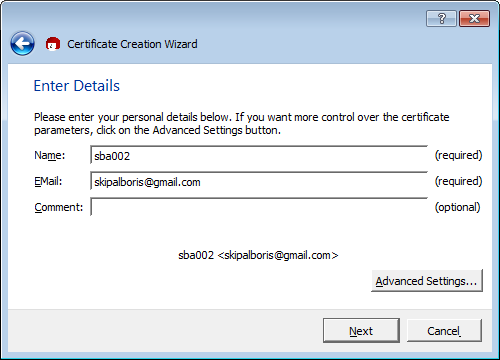
\includegraphics[width=1\linewidth]{res/step12}}
	\caption{Окно ввода информации о пользователе.}
	\label{ris:step12}
\end{figure}

После ввода личных данных необходимо ввести фразу-пароль (рисунок \ref{ris:step13}).

\begin{figure}[h]
	\center{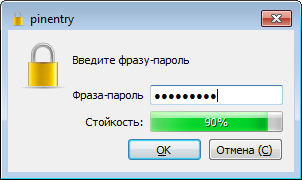
\includegraphics[width=0.6\linewidth]{res/step13}}
	\caption{Окно ввода фразы - пароля.}
	\label{ris:step13}

\end{figure}

После выполнения данных шагов, помощник выведет сообщение об успешном создании ключевой пары (рисунок \ref{ris:step14}).

\begin{figure}[h]
	\center{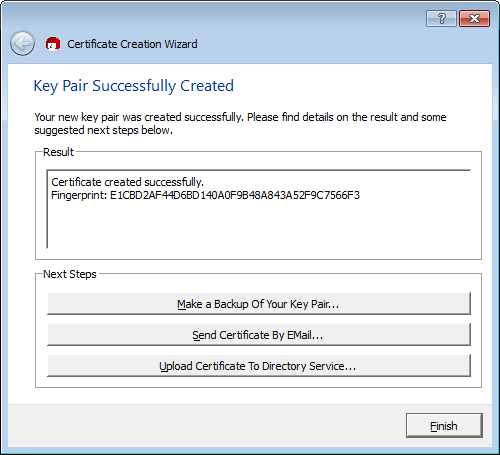
\includegraphics[width=1\linewidth]{res/step14}}
	\caption{Окно оповещения об успешном создании ключевой пары.}
	\label{ris:step14}
\end{figure}

Так же новая ключевая пара появится в рабочем пространстве (рисунок \ref{ris:step15}).

\begin{figure}[h]
	\center{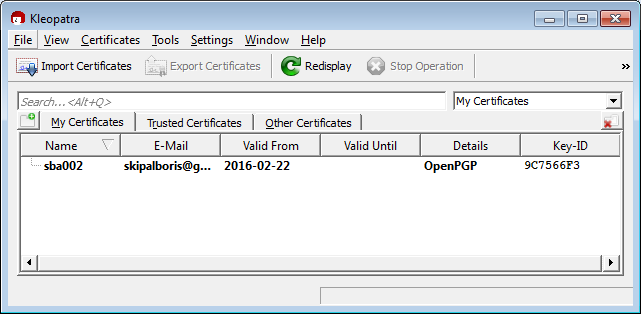
\includegraphics[width=1\linewidth]{res/step15}}
	\caption{Отображение новой ключевой пары.}
	\label{ris:step15}
\end{figure}

\subsection{Экспорт сертификата}
Для экспорта сертификата необходимо в графической оболочке \textit{"Kleopatra"} выполнить команду \textit{"File \begin{math}\to\end{math} Export Certificate"}. После чего откроется окно, в котором будет предложено выбрать название файла, где будет храниться сертификат (рисунок \ref{ris:step21})

\begin{figure}[h]
	\center{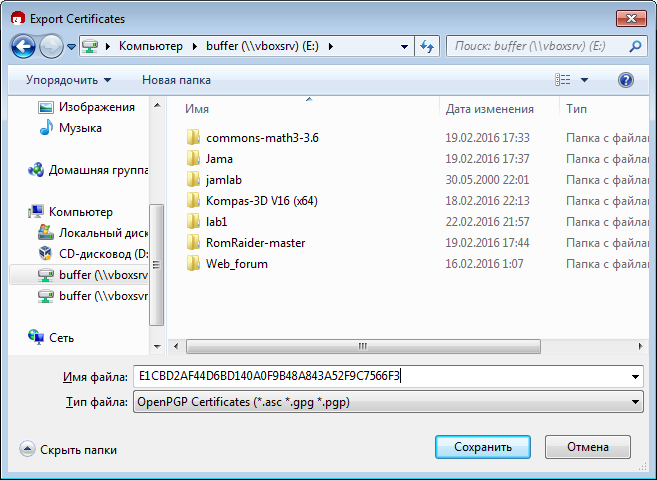
\includegraphics[width=1\linewidth]{res/step21}}
	\caption{Экспортирование сертификата.}
	\label{ris:step21}
\end{figure}

В данном случае файл будет называться\\"E1CBD2AF44D6BD140A0F9B48A843A52F9C7566F3.asc"

\subsection{Постановка ЭЦП на файл}
Перед тем, как поставить электронную цифровую подпись на файл, создадим текстовый файл "test.txt". Для того, что бы поставить свою ЭЦП на файл, необходимо выполнить команду \textit{"File \begin{math}\to\end{math} Sign/Encrypt Files"}. После чего появится окошко, в котором необходимо выбрать файл, для которого будет создаваться ЭЦП (рисунок \ref{ris:step31}).

\begin{figure}[h]
	\center{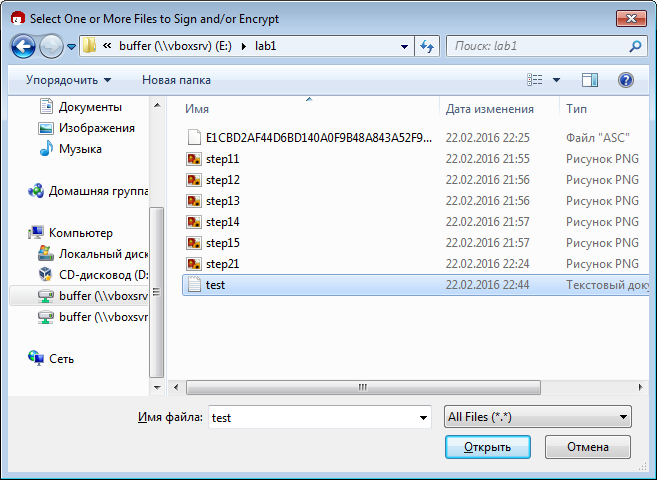
\includegraphics[width=1\linewidth]{res/step31}}
	\caption{Окно выбора файла.}
	\label{ris:step31}
\end{figure}

После чего помощника (рисунок \ref{ris:step32}), в котором необходимо выбрать пункт \textit{"Sign"} - создание цифровой подписи.

\begin{figure}[h]
	\center{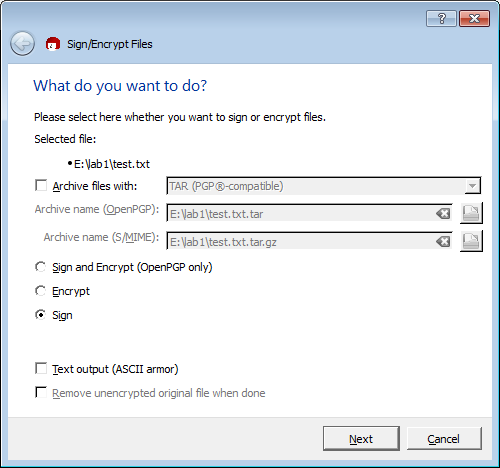
\includegraphics[width=1\linewidth]{res/step32}}
	\caption{Помощник создания ЭЦП.}
	\label{ris:step32}
\end{figure}

После чего появляется окошко, где необходимо подтвердить сертификат, которым будет подписываться файл (рисунок \ref{ris:step33}).

\begin{figure}[h]
	\center{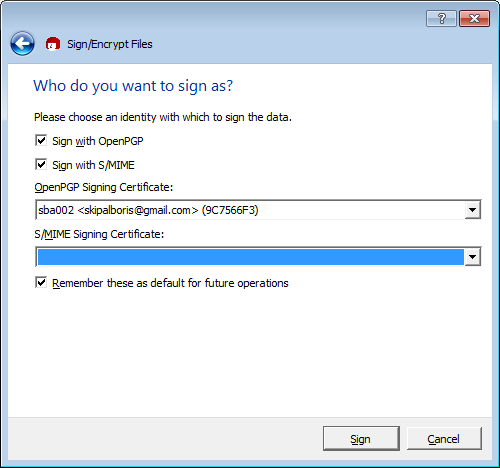
\includegraphics[width=1\linewidth]{res/step33}}
	\caption{Окно подтверждения сертификата.}
	\label{ris:step33}
\end{figure}

Затем необходимо аутентифицироваться при помощи пароля, заданного при создании ключа (рисунок \ref{ris:step34}).

\begin{figure}[h]
	\center{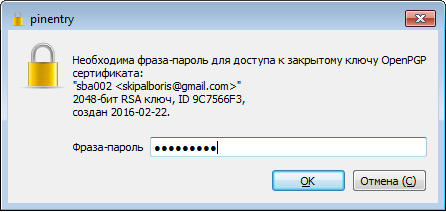
\includegraphics[width=0.7\linewidth]{res/step34}}
	\caption{Окно ввода пароля.}
	\label{ris:step34}
\end{figure}

После чего появится сообщение об успешном создании подписи (рисунок \ref{ris:step35}), а так же появится файл \textit{test.txt.sig}, в котором будет сохранена подпись.

\begin{figure}[h]
	\center{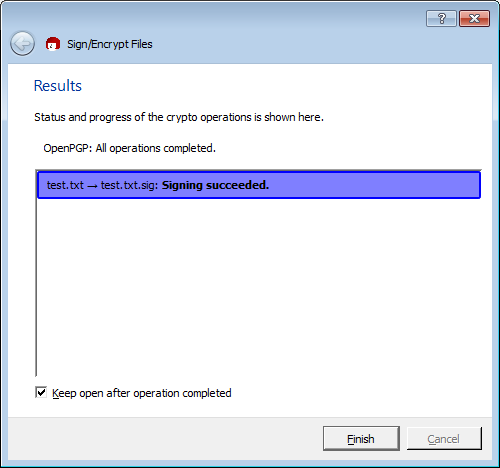
\includegraphics[width=1\linewidth]{res/step35}}
	\caption{Окно успешного создания подписи.}
	\label{ris:step35}
\end{figure}

Для проверки соответствия подписи выберем команду \textit{"File \begin{math}\to\end{math} Descript/ Verify Files"}. После чего необходимо выбрать сертификат, файл, который мы хотим проверить (в нашем случае test.txt), а так же файл с подписью (в нашем случае test.txt.sig). В случае успеха появится окошко, представленное на рисунке \ref{ris:step36}.

\begin{figure}[h]
	\center{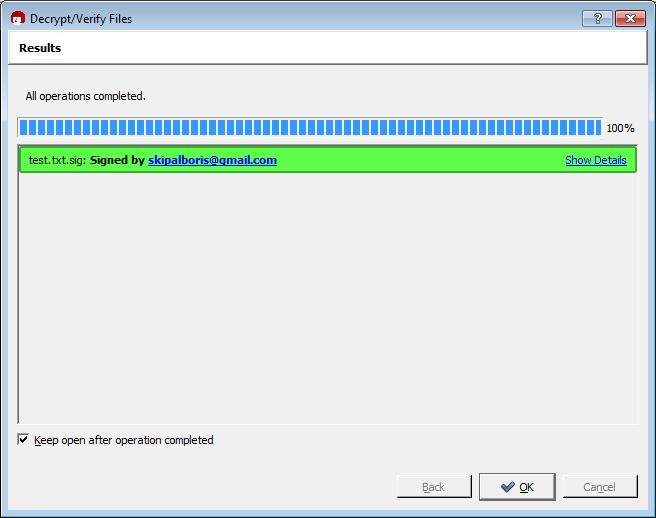
\includegraphics[width=1\linewidth]{res/step36}}
	\caption{Окно с результатами проверки подписи.}
	\label{ris:step36}
\end{figure}

\subsection{Импорт чужого сертификата}
Для импортирования чужого сертификата необходимо выполнить команду \textit{"File \begin{math}\to\end{math} Import Certificates"}. После чего откроется окно проводника, в котором необходимо выбрать чужой сертификат  (рисунок \ref{ris:step41}).

\begin{figure}[h]
	\center{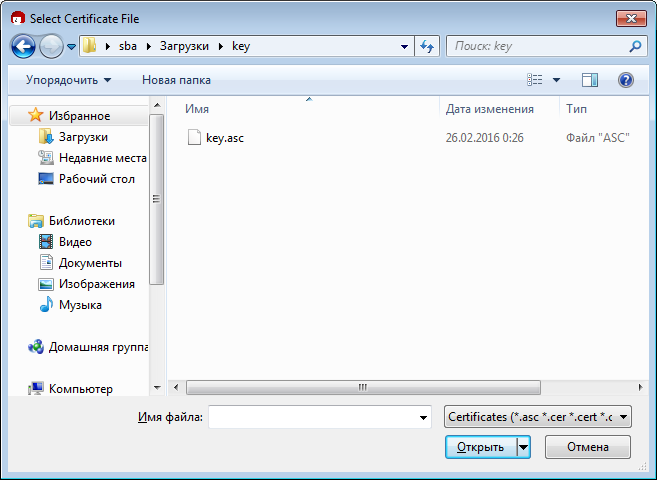
\includegraphics[width=1\linewidth]{res/step41}}
	\caption{Окно выбора файла сертификата.}
	\label{ris:step41}
\end{figure}

После этого новый сертификат можно увидеть во вкладке "Imported Certificates"  (рисунок \ref{ris:step42}).

\begin{figure}[h]
	\center{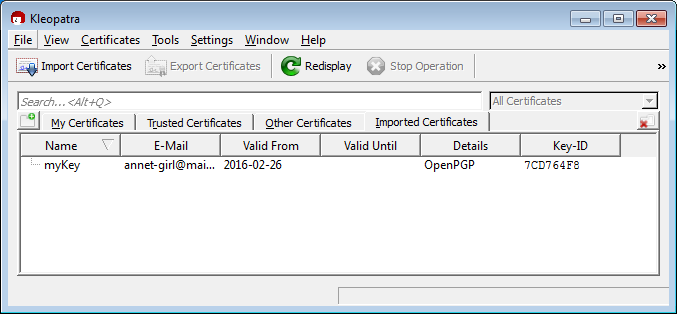
\includegraphics[width=1\linewidth]{res/step42}}
	\caption{Вкладка Imported Certificates.}
	\label{ris:step42}
\end{figure}

Для подписания чужого сертификата необходимо выполнить команду \textit{"File \begin{math}\to\end{math} Sign/ Encrypt Files"}. После чего появится окошко, в котором необходимо выбрать файл, для которого будет создаваться ЭЦП (в нашем случае необходимо указать сертификат другого человека). После чего для проверки необходимо выполнить пункт \textit{"File \begin{math}\to\end{math} Descript/ Verify Files"}. Результат представлен на рисунке \ref{ris:step43}.

\begin{figure}[h]
	\center{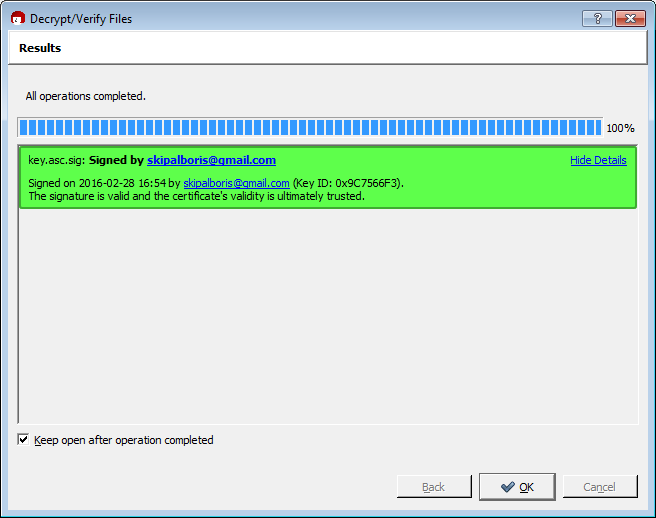
\includegraphics[width=1\linewidth]{res/step43}}
	\caption{Проверка подписи сертификата.}
	\label{ris:step43}
\end{figure}

\subsection{Использование консольных команд}
Вывод всех сертификатов происходит при помощи ключа  "\--list-keys".
\begin{verbatim}
	C:\Users\sba>gpg --list-keys
	C:/Users/sba/AppData/Roaming/gnupg/pubring.gpg
	----------------------------------------------
	pub   2048R/9C7566F3 2016-02-22
	uid     [абсолютное] sba002 <skipalboris@gmail.com>
	sub   2048R/00808598 2016-02-22
	
	pub   2048R/7CD764F8 2016-02-25
	uid     [неизвестно] myKey <annet-girl@mail.ru>
	sub   2048R/4BECA6BD 2016-02-25
\end{verbatim}

Для симметричного шифрования файла используется ключ "\--symmetric". Создадим файл "SkripalSec.txt" и зашифруем его при помощи закрытого ключа.

\begin{verbatim}
	gpg --symmetric SkripalSec.txt
\end{verbatim}

После этого в папке появится файл SkripalSec.txt.gpg

\begin{verbatim}
dir

28.02.2016  17:20    <DIR>          .
28.02.2016  17:20    <DIR>          ..
28.02.2016  16:52                 7 SkripalSec.txt
28.02.2016  17:20                60 SkripalSec.txt.gpg
\end{verbatim}

Для расшифровки файла необходимо использовать ключ "\--decrypt".

\begin{verbatim}
C:\Users\sba\Downloads\lab1>gpg --decrypt SkripalSec.txt.gpg
gpg: данные зашифрованы алгоритмом CAST5
gpg: зашифровано одной фразой-паролем
Hello!
gpg: ВНИМАНИЕ: целостность сообщения не защищена
\end{verbatim}
	
\end{document}